%---------------------------------------------------------------
\chapter{\babLima}
%---------------------------------------------------------------

%---------------------------------------------------------------
\section{Hasil Pengolahan Data Jarak}
%---------------------------------------------------------------
Pada bagian ini, data dari \textit{beat frequency} akan disajikan dalam bentuk gambar. Data tersebut adalah hasil setelah diolah pada langkah pengolahan data. Setelah didapat nilai \textit{beat frequency}, selanjutnya dimasukkan kedalam fungsi \textit{beat2range} yang terdapat pada matlab.

\subsection{Data Jarak 3 Meter}

\begin{figure}
    \centering
    \begin{subfigure}[b]{0.45\textwidth}
        \centering
        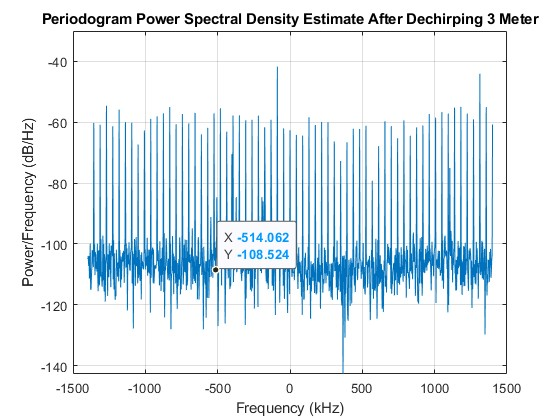
\includegraphics[scale=0.35]{pics/bab5/Range/1_3.jpg}
        \caption{Nilai \textit{beat frequency} 3 meter pengulangan 1}
        \label{fig:pengambilan3_1}
    \end{subfigure}
    \hfill
    \begin{subfigure}[b]{0.45\textwidth}
        \centering
        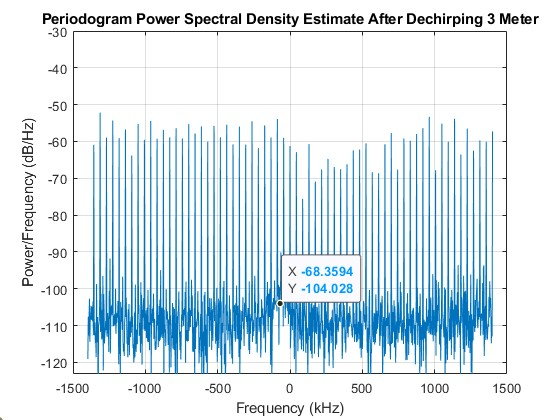
\includegraphics[scale=0.35]{pics/bab5/Range/2_3.jpg}
        \caption{Nilai \textit{beat frequency} 3 meter pengulangan 2}
        \label{fig:pengambilan3_2}
    \end{subfigure}
    \vskip\baselineskip
    \begin{subfigure}[b]{0.6\textwidth}
        \centering
        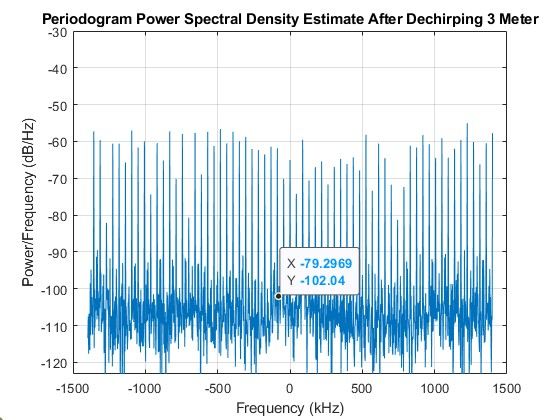
\includegraphics[scale=0.35]{pics/bab5/Range/3_3.jpg}
        \caption{Nilai \textit{beat frequency} 3 meter pengulangan 3}
        \label{fig:pengambilan3_3}
    \end{subfigure}
    \caption{Hasil \textit{beat frequency} dari jarak 3 meter}
    \label{fig:pengambilan3}
\end{figure}

Pada gambar~\ref{fig:pengambilan3} telah dilampirkan tiga sampel hasil percobaan dari total sembilan pengambilan data jarak objek setelah diolah dengan matlab untuk mendapatkan nilai \textit{beat frequency} dari objek. Pada gambar~\ref{fig:pengambilan3_1} yang menunjukkan pengambilan data pengulangan pertama didapatkan hasil nilai \textit{beat frequency} pada frekuensi -514.062 Hz, pada gambar~\ref{fig:pengambilan3_2} yang menunjukkan pengambilan data pengulangan kedua didapatkan nilai -68.3594 Hz, dan pada pengambilan data pengulangan ketiga, nilai \textit{beat frequency} adalah -79.2969 Hz seperti pada gambar~\ref{fig:pengambilan3_3}.

Dengan menggunakan persamaan~\ref{eq:RangeEst}, konversi \textit{beat frequency} ke jarak dapat dilakukan, perhitungan konversi adalah sebagai berikut.

\begin{align*}
    d_{0} &= \frac{|-514.062| \cdot 3 \cdot 10^{8}}{2 \cdot (\frac{14 \cdot 10^{6}}{0.01})}\\
   d_{0} &= 55.08 \phantom{b} meter\\
   d_{1} &= \frac{|-68.3594| \cdot 3 \cdot 10^{8}}{2 \cdot (\frac{14 \cdot 10^{6}}{0.01})}\\
   d_{1} &= 7.32 \phantom{b} meter\\
   d_{2} &= \frac{|-79.2969| \cdot 3 \cdot 10^{8}}{2 \cdot (\frac{14 \cdot 10^{6}}{0.01})}\\
   d_{2} &= 8.5 \phantom{b} meter\\
\end{align*}

Penggunaan mutlak pada \textit{beat frequency} karena nilai jarak yang didapat adalah nilai absolut yang merepresentasikan jarak di depan radar, dengan penggunaan \textit{double sideband} pada gambar~\ref{fig:pengambilan3Meter} maka \textit{beat frequency} perlu di ubah agar tidak mendapatkan hasil negatif jarak.

Konversi dari nilai \textit{beat frequency} menuju jarak dilakukan dengan fungsi \textit{beat2range} pada matlab, didapat dari nilai \textit{beat frequency} gambar~\ref{fig:pengambilan3_1} bahwa nilai jarak yang didapat adalah 55.08 meter. Nilai jarak dari \textit{beat frequency} gambar~\ref{fig:pengambilan3_2} adalah 7.32 meter. Sedangkan pada gambar~\ref{fig:pengambilan3_3} nilai jarak ada pada 8.50 meter. Dapat dilihat bahwa pada ketiga pengujian, nilai prediksi jarak tidak linier dengan jarak asli. Hal ini menunjukkan kegagalan radar dalam memprediksi jarak objek pada 3 meter.

\subsection{Data Jarak 6 Meter}

\begin{figure}
    \centering
    \begin{subfigure}[b]{0.45\textwidth}
        \centering
		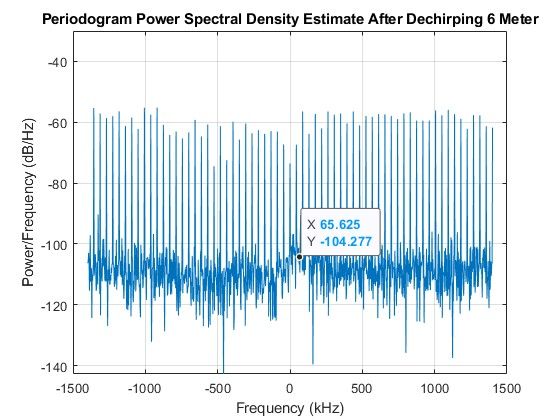
\includegraphics[scale=0.35]{pics/bab5/Range/1_6.jpg}
		\caption{Nilai \textit{beat frequency} 6 meter pengulangan 1}
		\label{fig:pengambilan6_1}
    \end{subfigure}
    \hfill
    \begin{subfigure}[b]{0.45\textwidth}
        \centering
		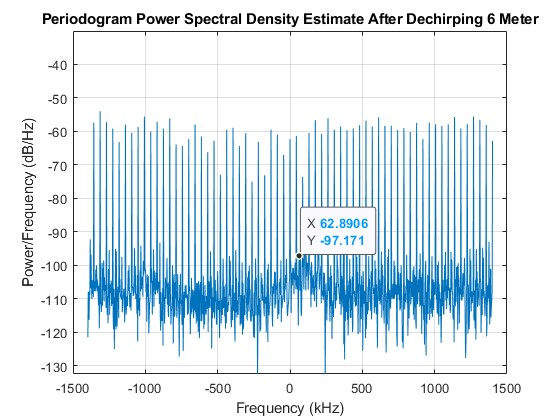
\includegraphics[scale=0.35]{pics/bab5/Range/2_6.jpg}
		\caption{Nilai \textit{beat frequency} 6 meter pengulangan 2}
		\label{fig:pengambilan6_2}
    \end{subfigure}
    \vskip\baselineskip
    \begin{subfigure}[b]{0.6\textwidth}
        \centering
		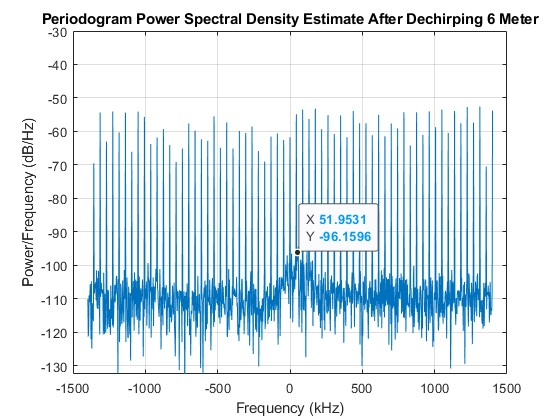
\includegraphics[scale=0.35]{pics/bab5/Range/3_6.jpg}
		\caption{Nilai \textit{beat frequency} 6 meter pengulangan 3}
		\label{fig:pengambilan6_3}
    \end{subfigure}
    \caption{Hasil \textit{beat frequency} dari jarak 6 meter}
    \label{fig:pengambilan6}
\end{figure}

Pada gambar~\ref{fig:pengambilan6} telah dilampirkan tiga dari sembilan sampel hasil percobaan pengambilan data jarak objek setelah diolah dengan matlab untuk mendapatkan nilai \textit{beat frequency} dari objek. Pada gambar~\ref{fig:pengambilan6_1} yang menunjukkan pengambilan data pengulangan pertama didapatkan hasil nilai \textit{beat frequency} pada frekuensi 65.625 Khz, pada gambar~\ref{fig:pengambilan6_2} yang menunjukkan pengambilan data pengulangan kedua didapatkan nilai 62.8906 kHz, dan pada pengambilan data pengulangan ketiga, nilai \textit{beat frequency} adalah 51.9531 kHz seperti pada gambar~\ref{fig:pengambilan6_3}.

Dengan menggunakan persamaan~\ref{eq:RangeEst} yang terkandung dalam fungsi yang tersedia pada matlab, maka didapat nilai jarak dari~\ref{fig:pengambilan6_1} adalah 7.03 meter. Pada hasil \textit{beat frequency} gambar~\ref{fig:pengambilan6_2}, konversi jarak yang didapat adalah 6.74 meter. Pada hasil pengujian ketiga seperti gambar~\ref{fig:pengambilan6_3}, hasil prediksi jarak adalah 5.57 meter. Dari hasil jarak yang sudah didapat, menunjukkan bahwa hasil prediksi radar bekerja dengan cukup baik. 

\subsection{Data Jarak 9 Meter}

\begin{figure}
    \centering
    \begin{subfigure}[b]{0.45\textwidth}
        \centering
		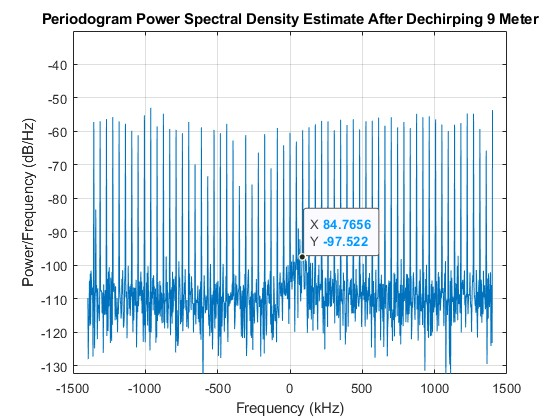
\includegraphics[scale=0.3]{pics/bab5/Range/1_9.jpg}
		\caption{Nilai \textit{beat frequency} 9 meter pengulangan 1}
		\label{fig:pengambilan9_1}
    \end{subfigure}
    \hfill
    \begin{subfigure}[b]{0.45\textwidth}
        \centering
		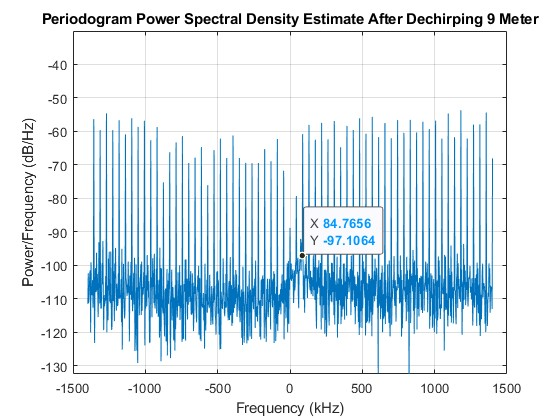
\includegraphics[scale=0.35]{pics/bab5/Range/2_9.jpg}
		\caption{Nilai \textit{beat frequency} 9 meter pengulangan 2}
		\label{fig:pengambilan9_2}
    \end{subfigure}
    \vskip\baselineskip
    \begin{subfigure}[b]{0.6\textwidth}
        \centering
		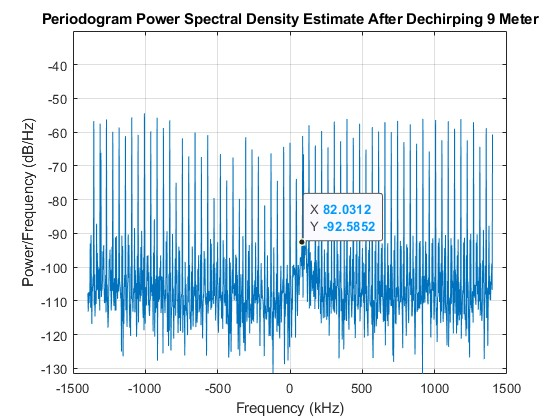
\includegraphics[scale=0.35]{pics/bab5/Range/3_9.jpg}
		\caption{Nilai \textit{beat frequency} 9 meter pengulangan 3}
		\label{fig:pengambilan9_3}
    \end{subfigure}
    \caption{Hasil \textit{beat frequency} dari jarak 9 meter}
    \label{fig:pengambilan9}
\end{figure}

Pada gambar~\ref{fig:pengambilan9} telah dilampirkan tiga sampel dari total sembilan hasil percobaan pengambilan data jarak objek setelah diolah dengan matlab untuk mendapatkan nilai \textit{beat frequency} dari objek. Pada gambar~\ref{fig:pengambilan9_1} yang menunjukkan pengambilan data pengulangan pertama didapatkan hasil nilai \textit{beat frequency} pada frekuensi 84.7656 Khz, pada gambar~\ref{fig:pengambilan9_2} yang menunjukkan pengambilan data pengulangan kedua didapatkan nilai 84.7656 kHz, dan pada pengambilan data pengulangan ketiga, nilai \textit{beat frequency} adalah 82.0312 kHz seperti pada gambar~\ref{fig:pengambilan9_3}.

Setelah nilai \textit{beat frequency} tiap pengulangan didapat, maka dilakukanlah konversi dengan fungsi \textit{beat2range}. didapat hasil jarak dari gambar~\ref{fig:pengambilan9_1} adalah 9.08 meter. Pada pengujian dari \textit{beat frequency} gambar~\ref{fig:pengambilan9_2}, nilai jarak juga didapat 9.08 meter. Pada pengujian ketiga dengan \textit{beat frequency} seperti gambar~\ref{fig:pengambilan9_3}, nilai jarak yang didapat adalah 8.79 meter. Hasil pengujian jarak 9 meter dari objek dengan menggunakan radar menunjukkan kemampuan radar yang dirancang sudah cukup baik dalam memprediksi jarak objek.
%---------------------------------------------------------------
\section{Hasil Pengolahan Data Kecepatan}
%---------------------------------------------------------------

Hasil prediksi kecepatan didapat dengan melakukan perhitungan dari nilai prediksi jarak yang terdeteksi dalam suatu waktu. Dengan mengamati frekuensi hasil \textit{conjugate}, akan didapat perubahan jarak objek yang didapat. 

\subsection{Data Kecepatan 5 km/h}

\begin{figure}
    \centering
    \begin{subfigure}[b]{0.45\textwidth}
        \centering
		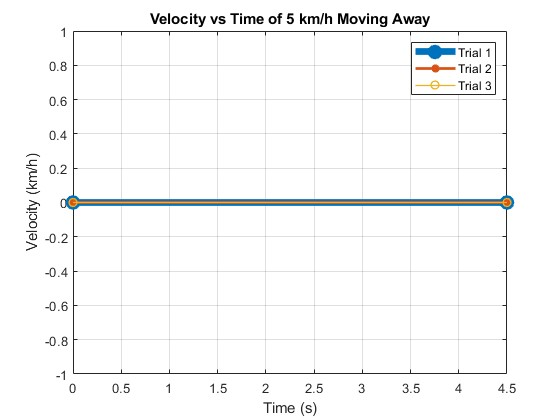
\includegraphics[scale=0.4]{pics/bab5/Velocity/5MA.jpg}
		\caption{Objek menjauhi radar}
		\label{fig:pengambilan5MA}
    \end{subfigure}
    \hfill
    \begin{subfigure}[b]{0.45\textwidth}
        \centering
		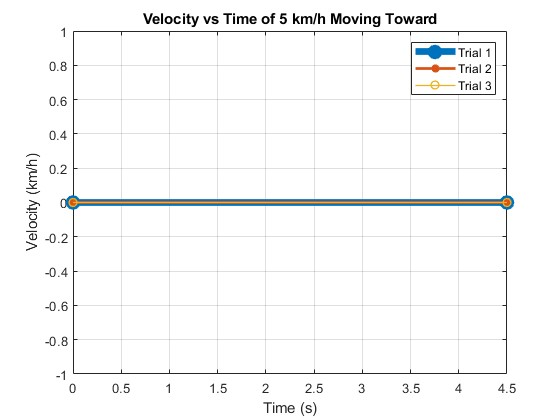
\includegraphics[scale=0.4]{pics/bab5/Velocity/5MT.jpg}
		\caption{Objek mendekati radar}
		\label{fig:pengambilan5MT}
    \end{subfigure}
    \caption{Hasil Prediksi Kecepatan Objek 5 km/h}
    \label{fig:pengambilan5}
\end{figure}

Pada gambar~\ref{fig:pengambilan5MA} dan gambar~\ref{fig:pengambilan5MT}, data kecepatan dari objek telah di ambil dan ditampilkan. Nampak bahwa data kecepatan tidak didapatkan. Hal ini sesuai dengan resolusi kecepatan yang telah dilampirkan dalam tabel~\ref{tab:spekRadar} bahwa objek baru akan terdeteksi setelah kecepatan mencapai minimal 9.31 km/h. 

\subsection{Data Kecepatan 10 km/h}

\begin{figure}
    \centering
    \begin{subfigure}[b]{0.45\textwidth}
        \centering
		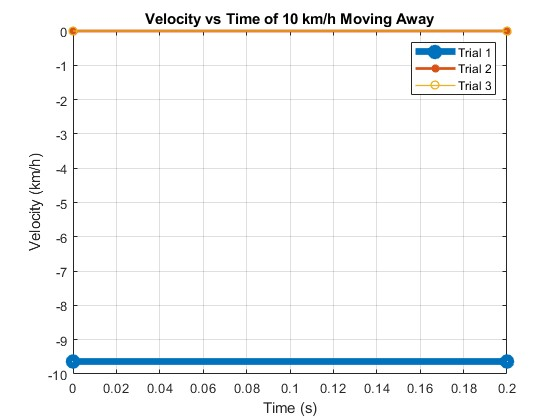
\includegraphics[scale=0.4]{pics/bab5/Velocity/10MA.jpg}
		\caption{Objek menjauhi radar}
		\label{fig:pengambilan10MA}
    \end{subfigure}
    \hfill
    \begin{subfigure}[b]{0.45\textwidth}
        \centering
		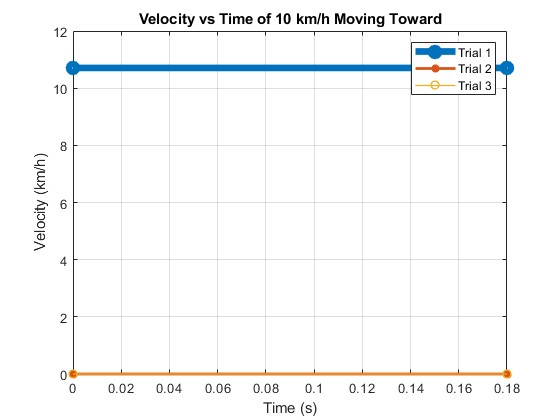
\includegraphics[scale=0.4]{pics/bab5/Velocity/10MT.jpg}
		\caption{Objek mendekati radar}
		\label{fig:pengambilan10MT}
    \end{subfigure}
    \caption{Hasil Prediksi Kecepatan Objek 10 km/h}
    \label{fig:pengambilan10}
\end{figure}

Data kecepatan dari objek bergerak telah di ambil dan ditampilkan pada gambar~\ref{fig:pengambilan10}. Grafik tersebut menunjukkan bahwa radar dapat melakukan hasil prediksi kecepatan dari objek. Dengan perbedaan paling mencolok dari kedua skema pengujian adalah saat objek menjauhi radar, maka nilai kecepatan ada pada negatif, sedangkan saat objek mendekati radar maka nilai kecepatan bernilai positif. Nilai prediksi kecepatan ada pada -9.8 km/h untuk objek menjauhi radar, sedangkan saat objek mendekati radar, nilai kecepatan terdeteksi adalah 10.3 km/h.

\subsection{Data Kecepatan 15 km/h}

\begin{figure}
    \centering
    \begin{subfigure}[b]{0.45\textwidth}
        \centering
		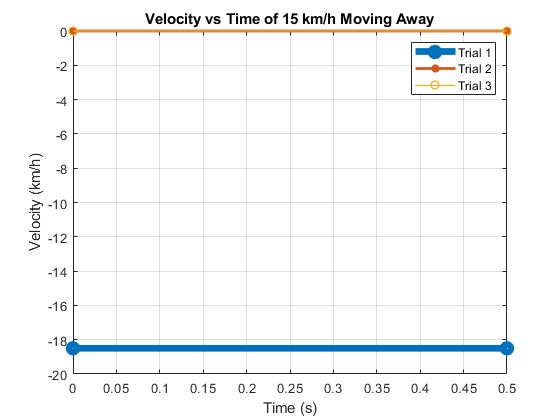
\includegraphics[scale=0.4]{pics/bab5/Velocity/15MA.jpg}
		\caption{Objek menjauhi radar}
		\label{fig:pengambilan15MA}
    \end{subfigure}
    \hfill
    \begin{subfigure}[b]{0.45\textwidth}
        \centering
		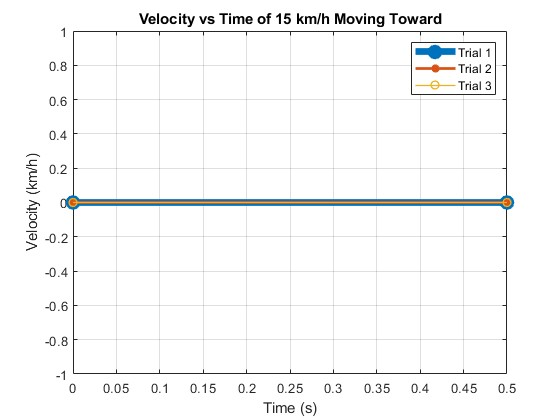
\includegraphics[scale=0.4]{pics/bab5/Velocity/15MT.jpg}
		\caption{Objek mendekati radar}
		\label{fig:pengambilan15MT}
    \end{subfigure}
    \caption{Hasil Prediksi Kecepatan Objek 15 km/h}
    \label{fig:pengambilan15}
\end{figure}

Gambar~\ref{fig:pengambilan15} menunjukkan hasil prediksi kecepatan objek 15 km/h. Dari kedua skema pengujian, hanya skema pengujian objek menjauhi radar yang terdeteksi. Pada prediksi kecepatan tersebut, nilai yang diprediksi adalah -18,03 km/h. Untuk objek yang mendekati radar, didapati bahwa kecepatan objek tidak terdeteksi. Sehingga dapat dinilai bahwa kemampuan radar untuk mendeteksi kecepatan objek pada kecepatan 15 km/h kurang baik.

\subsection{Data Kecepatan 20 km/h}

\begin{figure}
    \centering
    \begin{subfigure}[b]{0.45\textwidth}
        \centering
		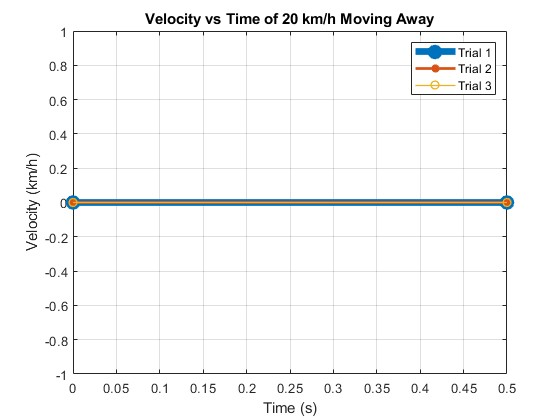
\includegraphics[scale=0.4]{pics/bab5/Velocity/20MA.jpg}
		\caption{Objek menjauhi radar}
		\label{fig:pengambilan20MA}
    \end{subfigure}
    \hfill
    \begin{subfigure}[b]{0.45\textwidth}
        \centering
		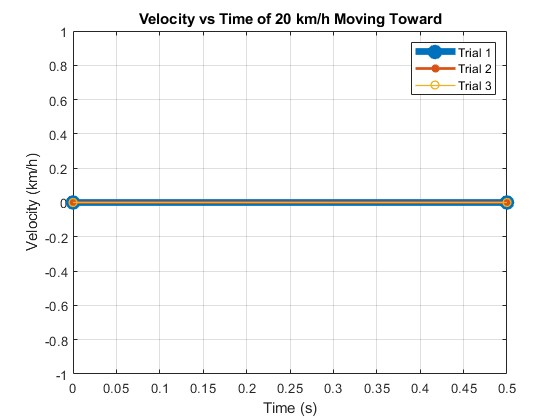
\includegraphics[scale=0.4]{pics/bab5/Velocity/20MT.jpg}
		\caption{Objek mendekati radar}
		\label{fig:pengambilan20MT}
    \end{subfigure}
    \caption{Hasil Prediksi Kecepatan Objek 20 km/h}
    \label{fig:pengambilan20}
\end{figure}

Data dari kecepatan objek yang bergerak pada kecepatan 20 km/h telah dilampirkan pada gambar~\ref{fig:pengambilan20}. Dapat dilihat bahwa kemampuan radar dalam mendeteksi objek yang bergerak pada kecepatan 20 km/h tidak bekerja. Baik pada skema pengujian objek mendekati maupun menjauhi radar. Maka dari itu, dapat dinyatakan bahwa kemampuan radar yang telah didesain tidak dapat mendeteksi objek dengan kecepatan 20 km/h.

%---------------------------------------------------------------
\section{Analisis Hasil}
%---------------------------------------------------------------

Pada tabel~\ref{tab:estRange} telah dilampirkan data deteksi jarak dari pengumpulan dan pengolahan data yang telah dilakukan. Pada tabel tersebut, didapatkan nilai deviasi antara prediksi dan nilai asli yang kecil pada jarak 6 meter dan 9 meter. Sedangkan pada data jarak 3 meter, didapati bahwa nilai prediksi sangat buruk.

\begin{table}[H]
    \caption{Tabel hasil prediksi dan akurasi}
    \label{tab:estRange}
    \begin{tabular}{|c|ccccccccc|c|}
    \hline
    \multirow{2}{*}{Jarak} & \multicolumn{9}{c|}{Hasil Prediksi}    & \multirow{2}{*}{Akurasi} \\ \cline{2-10}
                                & \multicolumn{1}{c|}{1}    & \multicolumn{1}{c|}{2}     & \multicolumn{1}{c|}{3}     & \multicolumn{1}{c|}{4}     & \multicolumn{1}{c|}{5}    & \multicolumn{1}{c|}{6}     & \multicolumn{1}{c|}{7}     & \multicolumn{1}{c|}{8}    & 9    &                          \\ \hline
    3                           & \multicolumn{1}{c|}{2,64} & \multicolumn{1}{c|}{53,61} & \multicolumn{1}{c|}{12,01} & \multicolumn{1}{c|}{8,50}  & \multicolumn{1}{c|}{3,22} & \multicolumn{1}{c|}{11,13} & \multicolumn{1}{c|}{55,08} & \multicolumn{1}{c|}{7,32} & 8,50 & -402,72 \%               \\ \hline
    6                           & \multicolumn{1}{c|}{6,74} & \multicolumn{1}{c|}{5,86}  & \multicolumn{1}{c|}{7,03}  & \multicolumn{1}{c|}{7,62}  & \multicolumn{1}{c|}{7,91} & \multicolumn{1}{c|}{7,62}  & \multicolumn{1}{c|}{7,03}  & \multicolumn{1}{c|}{6,74} & 5,57 & 82,86 \%                 \\ \hline
    9                           & \multicolumn{1}{c|}{9,67} & \multicolumn{1}{c|}{8,79}  & \multicolumn{1}{c|}{9,67}  & \multicolumn{1}{c|}{10,83} & \multicolumn{1}{c|}{7,62} & \multicolumn{1}{c|}{9,08}  & \multicolumn{1}{c|}{9,08}  & \multicolumn{1}{c|}{9,08} & 8,79 & 93,56 \%                 \\ \hline
    \end{tabular}

    \end{table}


Pada jarak 3 meter, didapat rata rata deviasi absolut sekitar 24.72 dengan nilai RMSE 2.72 dan nilai akurasi sekitar -402.72\%. Pada jarak pengujian 6 meter, didapatkan rata rata deviasi absolut sekitar 1.03 dengan nilai RMSE 1.17 dan nilai akurasi sekitar 82.86\%. Sedangkan pada jarak 9 meter, rata rata deviasi absolut adalah sekitar 0.58 dengan nilai RMSE 0.83 dan nilai akurasi sekitar 93.56\%. Maka dapat diambil suatu analisa bahwa kemampuan radar yang telah didesain bekerja sangat baik pada jarak 9 meter dan 6 meter. Sedangkan pada jarak 3 meter, radar yang telah didesain tidak dapat melakukan estimasi jarak objek.


\begin{table}[H]
    \caption{Hasil deteksi Kecepatan}
    \label{tab:estVelocity}
    \begin{tabular}{|c|cccccc|}
        \hline
        \multirow{3}{*}{Kecepatan} & \multicolumn{6}{c|}{Hasil Prediksi}                                                                                                                  \\ \cline{2-7} 
                                   & \multicolumn{3}{c|}{Menjauhi}                                                        & \multicolumn{3}{c|}{Mendekati}                                \\ \cline{2-7} 
                                   & \multicolumn{1}{c|}{1}           & \multicolumn{1}{c|}{2}  & \multicolumn{1}{c|}{3}  & \multicolumn{1}{c|}{1}         & \multicolumn{1}{c|}{2}  & 3  \\ \hline
        5                          & \multicolumn{1}{c|}{ND}          & \multicolumn{1}{c|}{ND} & \multicolumn{1}{c|}{ND} & \multicolumn{1}{c|}{ND}        & \multicolumn{1}{c|}{ND} & ND \\ \hline
        10                         & \multicolumn{1}{c|}{-9.8 KM/H}   & \multicolumn{1}{c|}{ND} & \multicolumn{1}{c|}{ND} & \multicolumn{1}{c|}{10.3 KM/H} & \multicolumn{1}{c|}{ND} & ND \\ \hline
        15                         & \multicolumn{1}{c|}{-18.03 KM/H} & \multicolumn{1}{c|}{ND} & \multicolumn{1}{c|}{ND} & \multicolumn{1}{c|}{ND}        & \multicolumn{1}{c|}{ND} & ND \\ \hline
        20                         & \multicolumn{1}{c|}{ND}          & \multicolumn{1}{c|}{ND} & \multicolumn{1}{c|}{ND} & \multicolumn{1}{c|}{ND}        & \multicolumn{1}{c|}{ND} & ND \\ \hline
        Akurasi                    & \multicolumn{3}{c|}{ND}                                                              & \multicolumn{3}{c|}{ND}                                       \\ \hline
        \end{tabular}
    \end{table}

Pada tabel~\ref{tab:estVelocity} telah dipaparkan beberapa sampel data hasil deteksi kecepatan objek yang bergerak. Bisa dilihat bahwa hasil estimasi kecepatan bisa berjalan, namun tidak dengan kemampuan yang baik. Arah dari gerakan objek yang bergerak juga dapat diamati. Pada saat objek bergerak menjauhi radar, nilai estimasi kecepatan akan negatif, sedangkan saat objek bergerak menjauhi radar, maka nilai estimasi kecepatan menjadi positif.

Karena hasil percobaan yang dapat dianalisis hasilnya hanyalah satu sampel, maka rata rata nilai absolut dan RMSE tidak bisa didapatkan. Sehingga dalam proses penilaian kualitas estimasi, kecepatan yang didapat hanya bisa dinilai dengan menggunakan deviasi absolut. Pada kecepatan 10 km/h mendekati radar, nilai deviasi adalah 0.3. Sedangkan saat objek bergerak menjauhi radar dengan kecepatan 10 km/h, didapatkan hasil negatif yang menunjukkan arah gerak objek, beserta nilai deviasi sekitar 0.2. Pengujian yang memiliki hasil selain dua di atas adalah pengujian 15 km/h yang memiliki nilai deviasi 3.03 dengan penunjuk arah negatif yang benar.

Alasan data hasil pengujian kecepatan sangat sulit untuk didapatkan dan diverifikasi karena penggunaan objek target berupa kendaraan bermotor roda dua. Dengan ukuran tersebut, maka dapat diasumsikan bahwa objek tersebut memiliki \textit{Radar Cross Section} yang tidak terlalu besar, yaitu sekitar $3 m^{2}$.